\documentclass[12pt, a4paper, simple]{eskdtext}

\usepackage{_env/gpi_global.env}
\usepackage{_env/gpi_report.env}
\usepackage{_sty/gpi_lst}
\usepackage{_sty/gpi_toc}
\usepackage{_sty/gpi_t}
\usepackage{_sty/gpi_u}

\def \gpiDocTopic {Отчёт лабораторной работы №\gpiDocNum}

\begin{document}
\begin{ESKDtitlePage}
    \ESKDstyle{empty}
    \begin{center}
        \gpiMinEduRep \\
        \gpiEduRep \\
        \gpiKafRep \\
    \end{center}

    \vfill

    \begin{center}
        Тема: <<\gpiTopicRep>>
    \end{center}

    \vfill

    \begin{center}
        \textbf{\gpiDocTopic} \\
        по дисциплине \gpiDisciplineRep \\
    \end{center}

    \vfill

    \begin{flushright}
        \begin{minipage}[t]{7cm}
            Выполнил: \\
            \PageTitleStudentInfo \\
            \hspace{0pt} \\
            Проверил: \\
            \PageTitleTeacherInfo \\
        \end{minipage}
    \end{flushright}

    \vfill

    \begin{center}
        \PageTitleCity~\ESKDtheYear
    \end{center}
\end{ESKDtitlePage}


\ESKDstyle{empty}

\begin{center}
    \textbf{\gpiDocTopic}
\end{center}

\paragraph{} \textbf{Тема}: <<\gpiTopicRep>>

\paragraph{} \textbf{Цель}:
изучить операторы ввода и вывода, форматы, используемые в этих операторах.
Разработать линейные алгоритмы и реализовать с применением этих операторов

\paragraph{} \textbf{Что нужно сделать}:

\begin{center}
    \textbf{Задание А5}
\end{center}

$\alpha = \ln{(y^{-\sqrt{|x|}})} * (x - y/2) + \sin^2{\arctan{(z)}}$

При $x = -15.246$, $y = 4.642*10^2$, $z = 20.001*10^2$ : $-182.036$.

\paragraph{} \textbf{Разработка алгоритма}:

Блок-схема изображена на рисунке~\ref{fig:a5}.

\begin{figure}[ph]
    \centering
    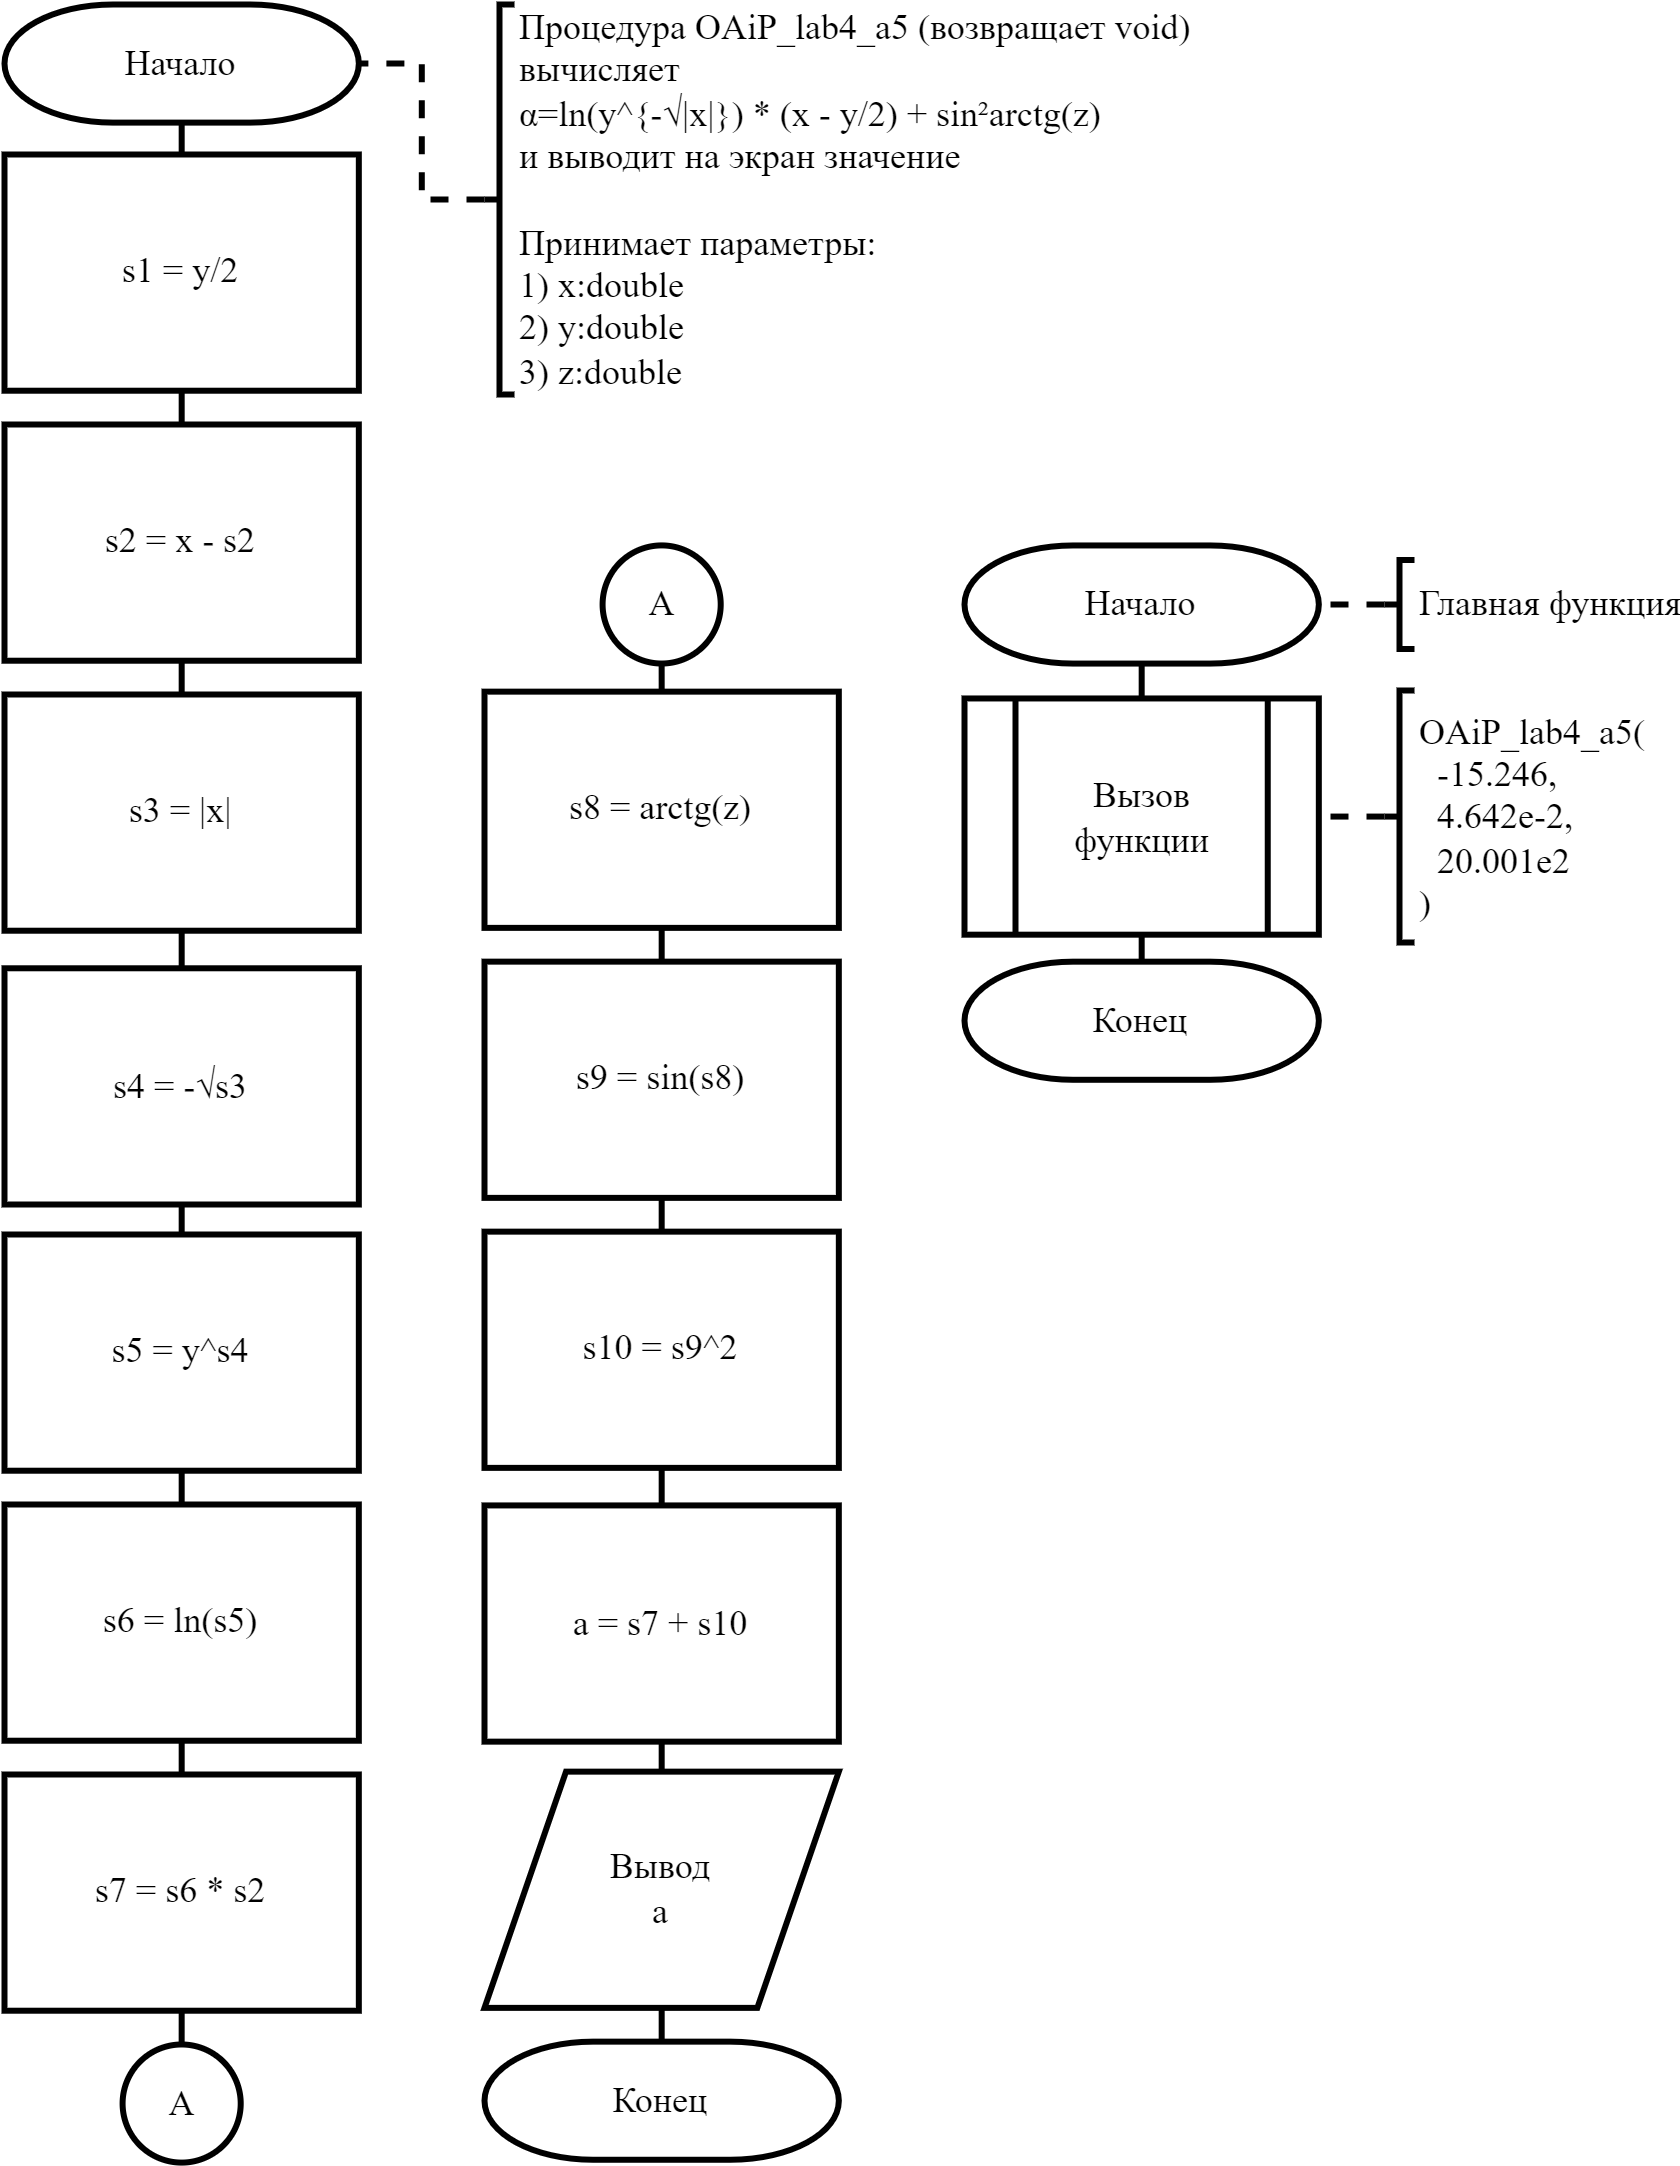
\includegraphics[]
    {../sources/flowcharts/OAiP_lab4_a5.png}
    \caption{Блок-схема}
    \label{fig:a5}
\end{figure}

\paragraph{} \textbf{Исходный код}: 

\lstinputlisting[language=c, name=main.cpp]
{../sources/OAiP_lab4_a5/OAiP_lab4_a5/main.cpp}

\begin{lstlisting}[name=Вывод в консоль]
-182.036
\end{lstlisting}

\paragraph{} \textbf{Что нужно сделать}:

\begin{center}
    \textbf{Задание Б5}
\end{center}

Даны два действительных числа x и y.
Вычислить их сумму, разность, произведение и частное.

\paragraph{} \textbf{Разработка алгоритма}:

Блок-схема изображена на рисунке~\ref{fig:b5}.

\begin{figure}[ph]
    \centering
    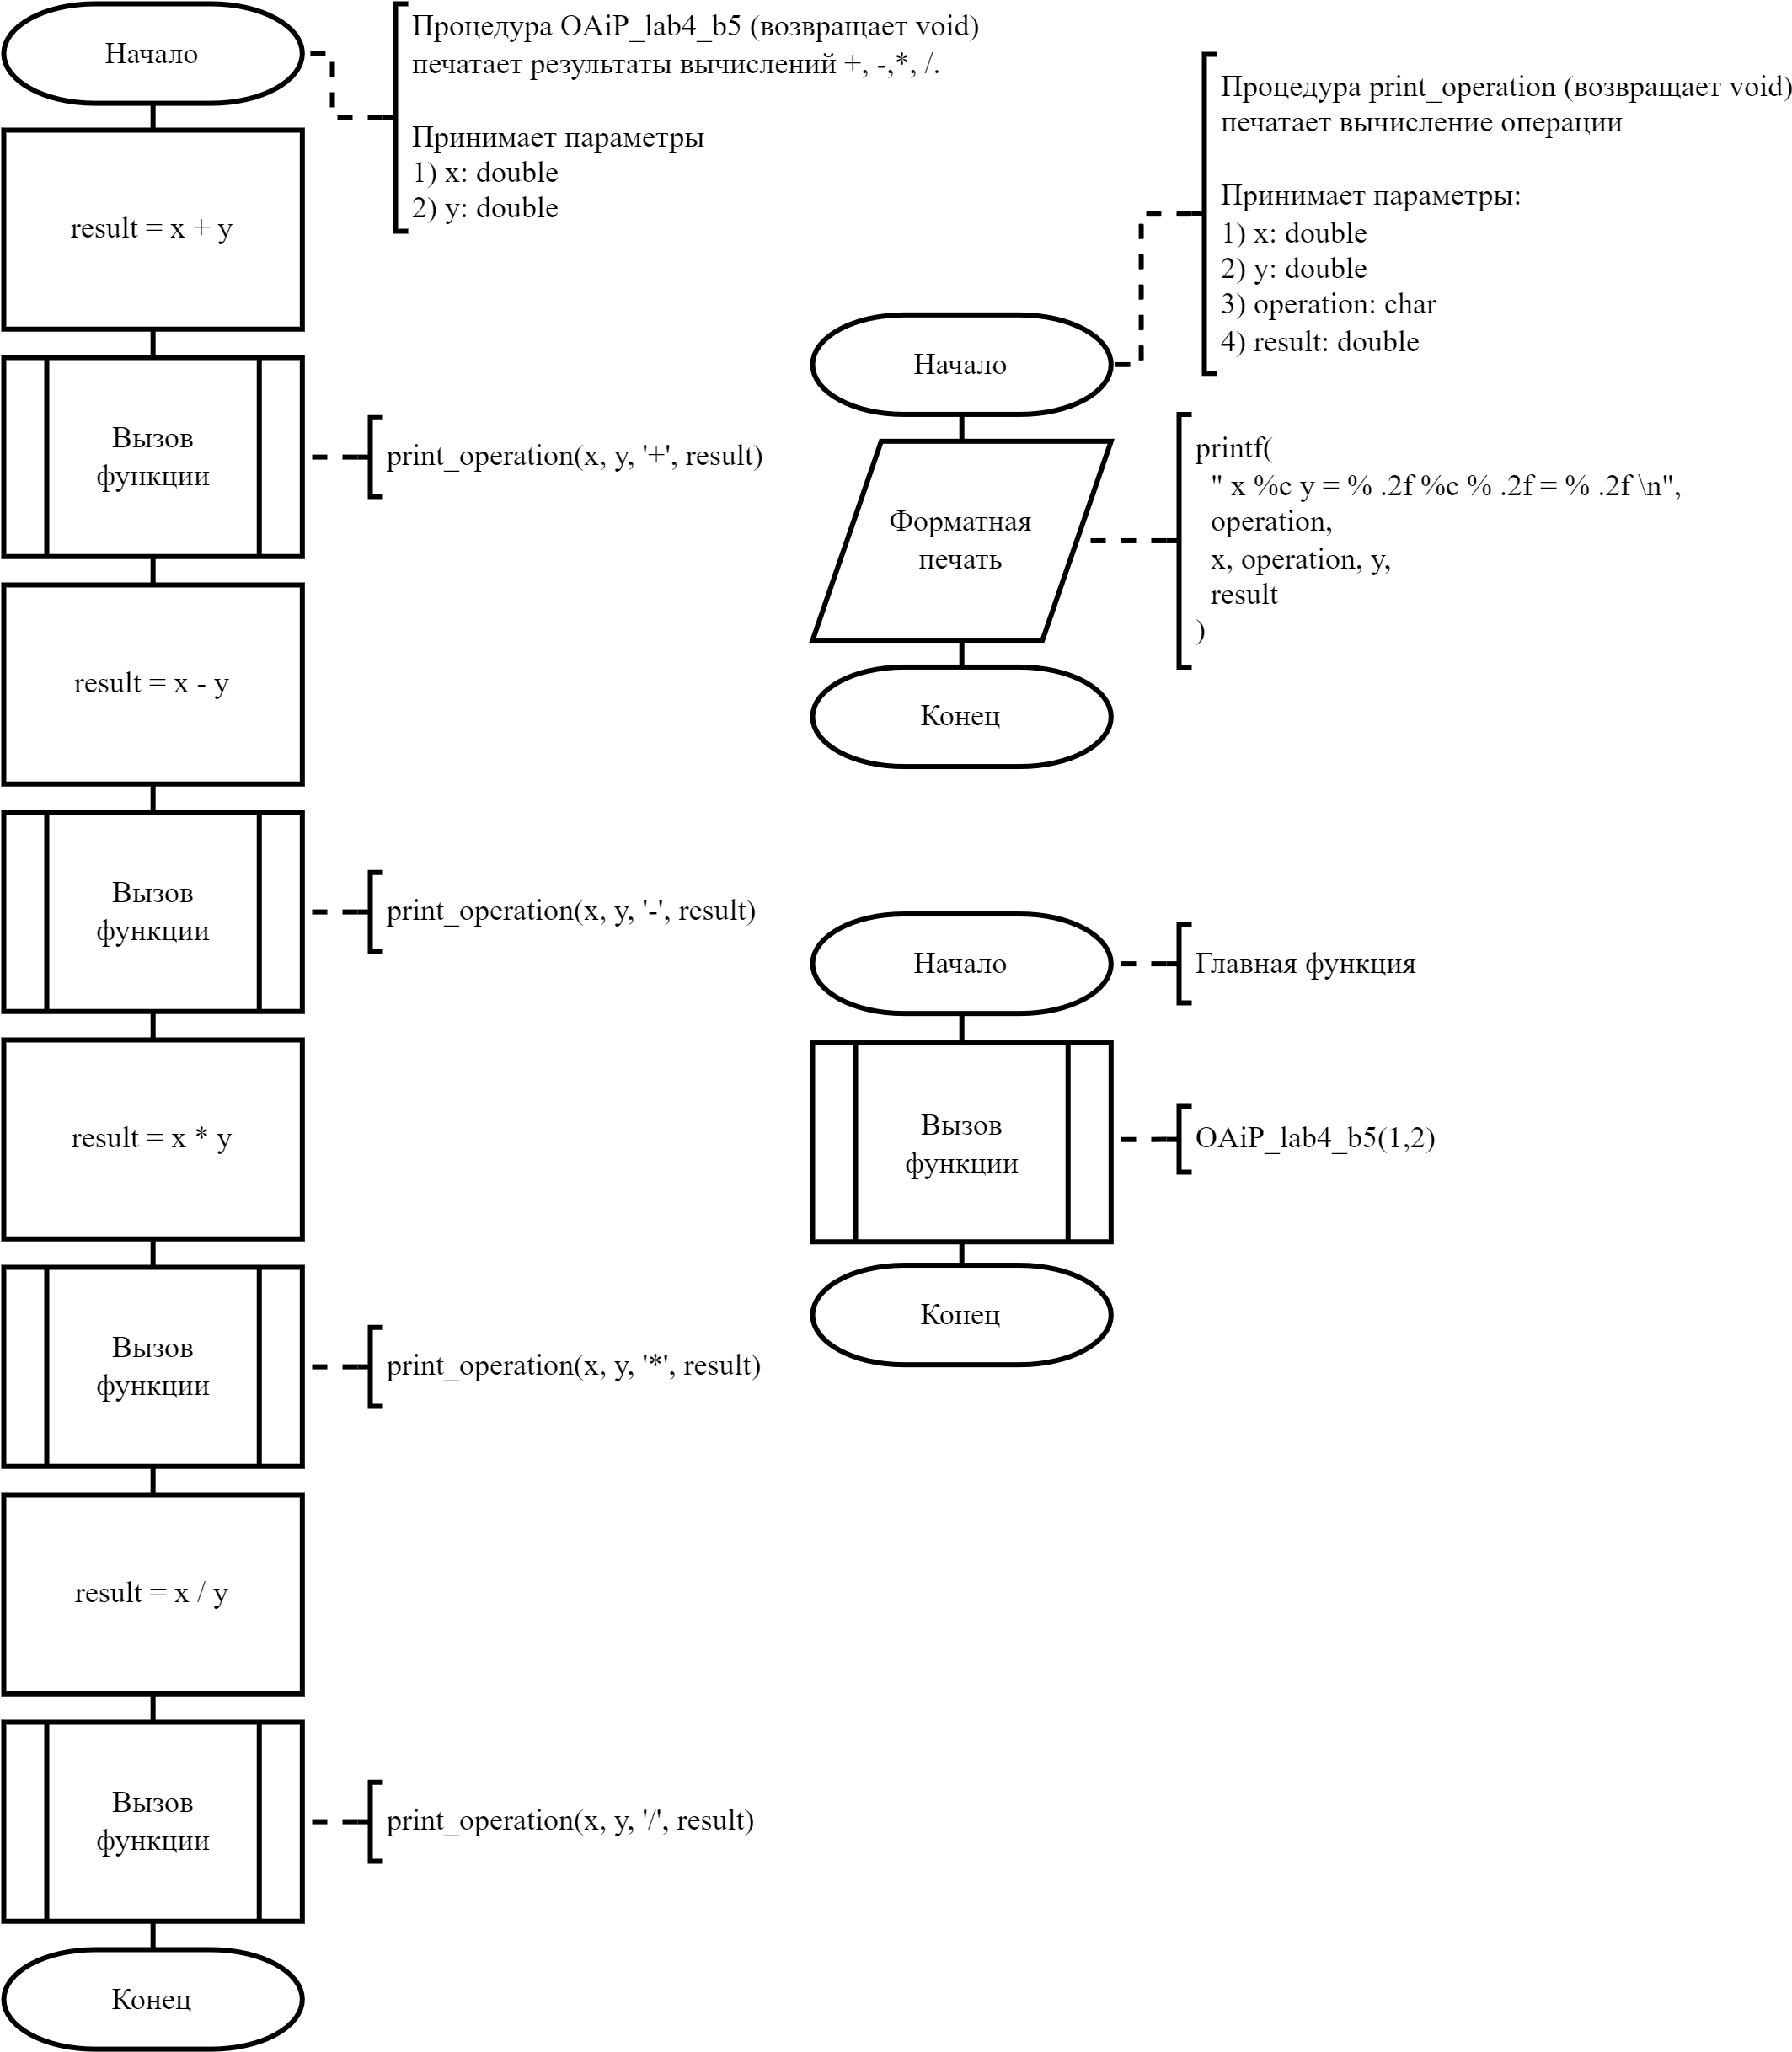
\includegraphics[]
    {../sources/flowcharts/OAiP_lab4_b5.png}
    \caption{Блок-схема}
    \label{fig:b5}
\end{figure}

\paragraph{} \textbf{Исходный код}: 

\lstinputlisting[language=c, name=main.cpp]
{../sources/OAiP_lab4_b5/OAiP_lab4_b5/main.cpp}


\begin{lstlisting}[name=Вывод в консоль]
 x + y =  1.00 +  2.00 =  3.00
 x - y =  1.00 -  2.00 = -1.00
 x * y =  1.00 *  2.00 =  2.00
 x / y =  1.00 /  2.00 =  0.50
\end{lstlisting}


\paragraph{} \textbf{Вывод}:
изучил операторы ввода и вывода, форматы, используемые в этих операторах.
Разрабол линейные алгоритмы и реализовал с применением этих операторов.


% = = = = = = = =
\newpage
% \addcontentsline{toc}{section}{Список использованных источников}
% \section*{Список использованных источников}
\paragraph{} \textbf{Список использованных источников}:
\begin{enumerate}
    \item[1.] Коллекция eskdx v0.98 - eskdx.pdf
    [Электронный ресурс].
    Режим доступа: \url{http://tug.ctan.org/macros/latex/contrib/eskdx/manual/eskdx.pdf}.
    Дата доступа: 30.05.2022.

    \item[2.] Использование системы верстки LaTeX - EVMiS\_Latex.pdf
    [Электронный ресурс].
    Режим доступа: \url{https://www.bstu.by/uploads/attachments/metodichki/kafedri/EVMiS_Latex.pdf}.
    Дата доступа: 30.05.2022.

    \item[3.] Опции пакета hyperref
    [Электронный ресурс].
    Режим доступа: \url{https://grammarware.net/text/syutkin/hyperref_options.pdf}.
    Дата~доступа:~20.02.2022.

    \item[4.] Developers - Docker
    [Electronic resource].
    Mode of access: \url{https://www.docker.com/get-started/}.
    Date~of~access:~04.06.2022.

    \item[5.] Manual installation steps for older versions of WSL | Microsoft Docs
    [Electronic resource].
    Mode of access: \url{https://aka.ms/wsl2kernel}.
    Date~of~access:~04.06.2022.

    \item[6.] LaTeX/Source Code Listings - Wikibooks, open books for an open world
    [Electronic resource].
    Mode of access: \url{https://en.wikibooks.org/wiki/LaTeX/Source_Code_Listings}.
    Date~of~access:~04.06.2022.

    \item[7.] LaTeX/Mathematics - Wikibooks, open books for an open world
    [Electronic resource].
    Mode of access: \url{https://en.wikibooks.org/wiki/LaTeX/Mathematics}.
    Date~of~access:~05.06.2022.

    \item[8.] 1sem\_OAiP/OAiP\_lab4.pdf at galanin · BrSTU-PO4-Galanin/1sem\_OAiP
    [Электронный ресурс].
    Режим доступа: \url{https://github.com/BrSTU-PO4-Galanin/1sem_OAiP/blob/galanin/docs/lab4/OAiP_lab4.pdf}.
    Дата доступа: 05.06.2022.
\end{enumerate}

\newpage
\end{document}
